\documentclass[11pt,a4paper]{article}

% Datos de la actividad
\newcommand{\codigoactividad}{FORM-TL-01}
\newcommand{\nombreactividad}{Taller de modelado de comunicación entre procesos distribuidos}
\newcommand{\escenario}{2 (plataforma de streaming OndaPlay)}
\newcommand{\integrantes}{Castro Coello Mario Sebastián \\ Loor Suárez Steffanny del Rocío \\ Quintero Rico Luis David \\ Rivas Piloso Dayver Yahir}
\newcommand{\repositorio}{https://github.com/reyshadow0/isr701-form-tl-01}
\newcommand{\fechaentrega}{11 de noviembre de 2026}

\usepackage[T1]{fontenc}
\usepackage[utf8]{inputenc}
\usepackage[spanish,es-tabla,es-nodecimaldot]{babel}
\usepackage{lmodern}
\usepackage{microtype}
\usepackage[a4paper,margin=2.5cm]{geometry}
\usepackage{graphicx}
\usepackage{booktabs}
\usepackage{tabularx}
\usepackage{float}
\usepackage{xcolor}
\usepackage{listings}
\usepackage{csquotes}
\usepackage[backend=biber,style=ieee]{biblatex}
\addbibresource{referencias.bib}
\usepackage[hidelinks]{hyperref}

\graphicspath{{diagrama/}}

% Permite cortar URL largas en la bibliografía (evita desbordes)
\setcounter{biburlnumpenalty}{100}
\setcounter{biburlucpenalty}{100}
\setcounter{biburllcpenalty}{100}

\lstset{
  basicstyle=\ttfamily\small,
  breaklines=true,
  frame=single,
  numbers=left,
  numberstyle=\tiny,
  showstringspaces=false,
  extendedchars=true,
  literate={á}{{\'a}}1 {é}{{\'e}}1 {í}{{\'i}}1 {ó}{{\'o}}1 {ú}{{\'u}}1
           {Á}{{\'A}}1 {É}{{\'E}}1 {Í}{{\'I}}1 {Ó}{{\'O}}1 {Ú}{{\'U}}1
           {ñ}{{\~n}}1 {Ñ}{{\~N}}1 {ü}{{\"u}}1 {¿}{{?`}}1 {¡}{{!`}}1
}
\renewcommand{\lstlistingname}{Código}

\hypersetup{pdftitle={\codigoactividad: \nombreactividad}}

\begin{document}

\begin{titlepage}
  \centering
  {\large\bfseries UNIVERSIDAD TÉCNICA ESTATAL DE QUEVEDO\par}
  \vspace{0.3cm}
  {Facultad de Ciencias de la Computación\par}
  {Carrera de Software\par}
  \vspace{2.5cm}
  {\large Aplicaciones Distribuidas (ISR-701)\par}
  \vspace{1.5cm}
  {\Large\bfseries \codigoactividad\par}
  \vspace{0.4cm}
  {\LARGE \nombreactividad\par}
  \vspace{1cm}
  {\large Notas del taller\par}
  \vspace{0.2cm}
  {\large Escenario: \escenario\par}
  \vfill
  \begin{tabular}{@{}rl@{}}
    \textbf{Integrantes:}      & \begin{tabular}[t]{@{}l@{}}\integrantes\end{tabular} \\[2pt]
    \textbf{Docente:}          & Gleiston Cicerón Guerrero Ulloa, PhD \\
    \textbf{Nivel / paralelo:} & Séptimo nivel / B \\
    \textbf{Periodo:}          & SPA 2026--2027 \\
    \textbf{Fecha:}            & \fechaentrega \\
  \end{tabular}
  \par\vspace{1cm}
  {\small Repositorio: \url{\repositorio}\par}
\end{titlepage}

\tableofcontents
\newpage

\section{Escenario y procesos}
\label{sec:escenario}

\subsection{Qué es OndaPlay}

El caso viene del enunciado del escenario 2 (Anexo A de la rúbrica
GA-TL-01). OndaPlay es un servicio de streaming ficticio, con
suscripción, que combina catálogo bajo demanda y eventos en vivo de
fin de semana, y que se ve desde el celular, la televisión o el
navegador. El rediseño parte de tres fallas actuales: arranque lento
del video en los eventos en vivo, reproducciones de usuarios sin
suscripción vigente y datos de visualización que llegan tarde al
equipo de recomendaciones.

\subsection{Actores y frontera del sistema}

El suscriptor usa el reproductor para iniciar sesión, buscar títulos,
ver contenido y renovar su plan. El administrador de contenidos carga
títulos, temporadas y metadatos en el catálogo. La pasarela de pagos
es un sistema externo que procesa los cobros de las suscripciones.

Dentro de la frontera quedan los procesos que OndaPlay controla: los
siete procesos mínimos, la puerta de enlace y el bróker de mensajes.
La pasarela de pagos queda fuera, y OndaPlay solo se comunica con ella
desde el servicio de facturación. Los servidores de borde de la CDN,
que el enunciado también lista como actor, se modelan dentro del sistema
como el proceso VID, porque son los que entregan el video al
reproductor.

\subsection{Procesos mínimos}

Cada proceso usa el mismo código que en el diagrama de la sección 2.

\begin{description}
  \item[CLI] Reproductor (cliente). Inicia sesión, muestra el catálogo,
    pide la licencia y los segmentos de video y envía la telemetría.
  \item[AUT] Servicio de autenticación y licencias. Verifica que la
    suscripción esté vigente y entrega la licencia para reproducir.
  \item[CAT] Servicio de catálogo. Guarda títulos, temporadas y
    metadatos.
  \item[VID] Servidor de contenido o nodo de borde. Entrega los
    segmentos de video al reproductor.
  \item[TEL] Servicio de telemetría. Recibe los eventos del
    reproductor: inicio, pausa, avance, errores y calidad.
  \item[REC] Servicio de recomendaciones. Consume los eventos de
    visualización para actualizar las recomendaciones de cada usuario.
  \item[PAG] Servicio de facturación y suscripciones. Registra
    renovaciones y cancelaciones, cobra a través de la pasarela de
    pagos y responde el estado de cada suscripción.
\end{description}

\subsection{Procesos agregados: GW y MSG}

GW es la puerta de enlace (API Gateway). Recibe las peticiones del
reproductor, las dirige a AUT o a CAT y devuelve la respuesta, así el
reproductor no necesita conocer la dirección de cada servicio interno.
También guarda en caché las consultas frecuentes del catálogo y
reintenta las llamadas a AUT cuando una instancia falla
(sección~\ref{sec:sincronas}). Los segmentos de video no pasan por
GW: el reproductor los pide directamente al nodo de borde.

MSG es el bróker de mensajes. Lo agregamos para los flujos que no
necesitan respuesta inmediata. TEL publica en MSG los eventos de
visualización y REC los consume a su ritmo. Si REC se cae, los eventos
quedan guardados en el bróker hasta que vuelva (F2). PAG usa el mismo
canal para avisar a AUT de una cancelación. Estos flujos se detallan
en la sección 4.

\subsection{Por qué la solución es distribuida}

Los procesos corren en máquinas distintas y se comunican solo por la
red, sin memoria compartida. El reproductor está en el dispositivo de
cada suscriptor, los nodos de borde se ubican cerca de los
espectadores, los servicios internos corren en el centro de datos de
OndaPlay y la pasarela de pagos pertenece a otra empresa.

Repartir el trabajo también responde a los requisitos. Un solo
servidor no atiende a 50\,000 espectadores simultáneos (R1), por eso
la carga se reparte entre varios nodos de borde. La disponibilidad
del 99,9\,\% de las licencias (R6) exige varias instancias de AUT. Y
como REC está separado del flujo de reproducción, una caída de las
recomendaciones no detiene el video.

\subsection{Operaciones del escenario}

\begin{itemize}
  \item[(a)] \emph{Iniciar sesión y explorar el catálogo.} Las
    búsquedas y la consulta de un título van de CLI a GW y de GW a
    CAT (S4).
  \item[(b)] \emph{Solicitar la licencia y empezar a reproducir.} GW
    pide la licencia a AUT (S2) y AUT consulta a PAG el estado de la
    suscripción (S3). Con el token de licencia, CLI pide los segmentos
    al nodo de borde VID (S1).
  \item[(c)] \emph{Enviar la telemetría mientras se reproduce.} CLI
    envía a TEL un evento cada 10 segundos.
  \item[(d)] \emph{Actualizar las recomendaciones a partir de lo
    visto.} TEL publica los eventos de visualización en MSG y REC los
    consume para recalcular las recomendaciones.
  \item[(e)] \emph{Renovar la suscripción y reflejar el cambio en las
    licencias.} PAG cobra a través de la pasarela de pagos, actualiza
    el estado de la suscripción y avisa a AUT, que usa el nuevo estado
    en las siguientes licencias.
\end{itemize}

\subsection{Requisitos y situaciones de fallo}

El enunciado del escenario 2 fija seis requisitos cuantificados y tres
situaciones de fallo (tabla~\ref{tab:requisitos}), y pide que el
diseño cumpla R2 y R4 a la vez. La guía agrega una restricción: al
menos una interacción con sockets y otra con RPC.

\begin{table}[H]
  \centering
  \small
  \caption{Requisitos cuantificados y situaciones de fallo de OndaPlay}
  \label{tab:requisitos}
  \begin{tabularx}{\textwidth}{@{}lX@{}}
    \toprule
    \textbf{Código} & \textbf{Descripción} \\
    \midrule
    R1 & En una transmisión en vivo puede haber 50\,000 espectadores
         simultáneos. \\
    R2 & El video debe empezar a reproducirse en menos de 2 segundos
         desde que el usuario pulsa «reproducir», incluida la
         verificación de la licencia. \\
    R3 & Cada reproductor envía un evento de telemetría cada
         10 segundos; en una transmisión en vivo son unos 5\,000
         eventos por segundo. Se acepta perder hasta el 1\,\% de esos
         eventos. \\
    R4 & Una suscripción vencida o cancelada debe impedir nuevas
         reproducciones en menos de 5 minutos. \\
    R5 & Las recomendaciones pueden actualizarse con hasta 15 minutos
         de retraso (consistencia eventual aceptable). \\
    R6 & El servicio de licencias debe tener una disponibilidad del
         99,9\,\%, porque sin licencia no hay reproducción. \\
    \midrule
    F1 & El servicio de licencias no responde: ¿se bloquea a todos los
         usuarios o se permite reproducir durante un tiempo? \\
    F2 & El servicio de recomendaciones está caído durante dos horas:
         ¿se pierden los eventos de visualización de ese periodo? \\
    F3 & Un nodo de borde falla en plena transmisión en vivo: ¿qué pasa
         con los espectadores conectados a él? \\
    \bottomrule
  \end{tabularx}
\end{table}


\section{Diagrama de comunicación entre procesos}

El diagrama de OndaPlay muestra cómo se comunican los
procesos que intervienen en el funcionamiento de esta
plataforma de streaming. En él se representan los
servicios que participan en las solicitudes del cliente,
la verificación de licencias y suscripciones, la consulta
del catálogo y el acceso al contenido audiovisual.

La Figura~\ref{fig:diagrama} presenta los procesos
de OndaPlay, sus interacciones y los actores externos
que participan en el sistema.

\begin{figure}[H]
    \centering
    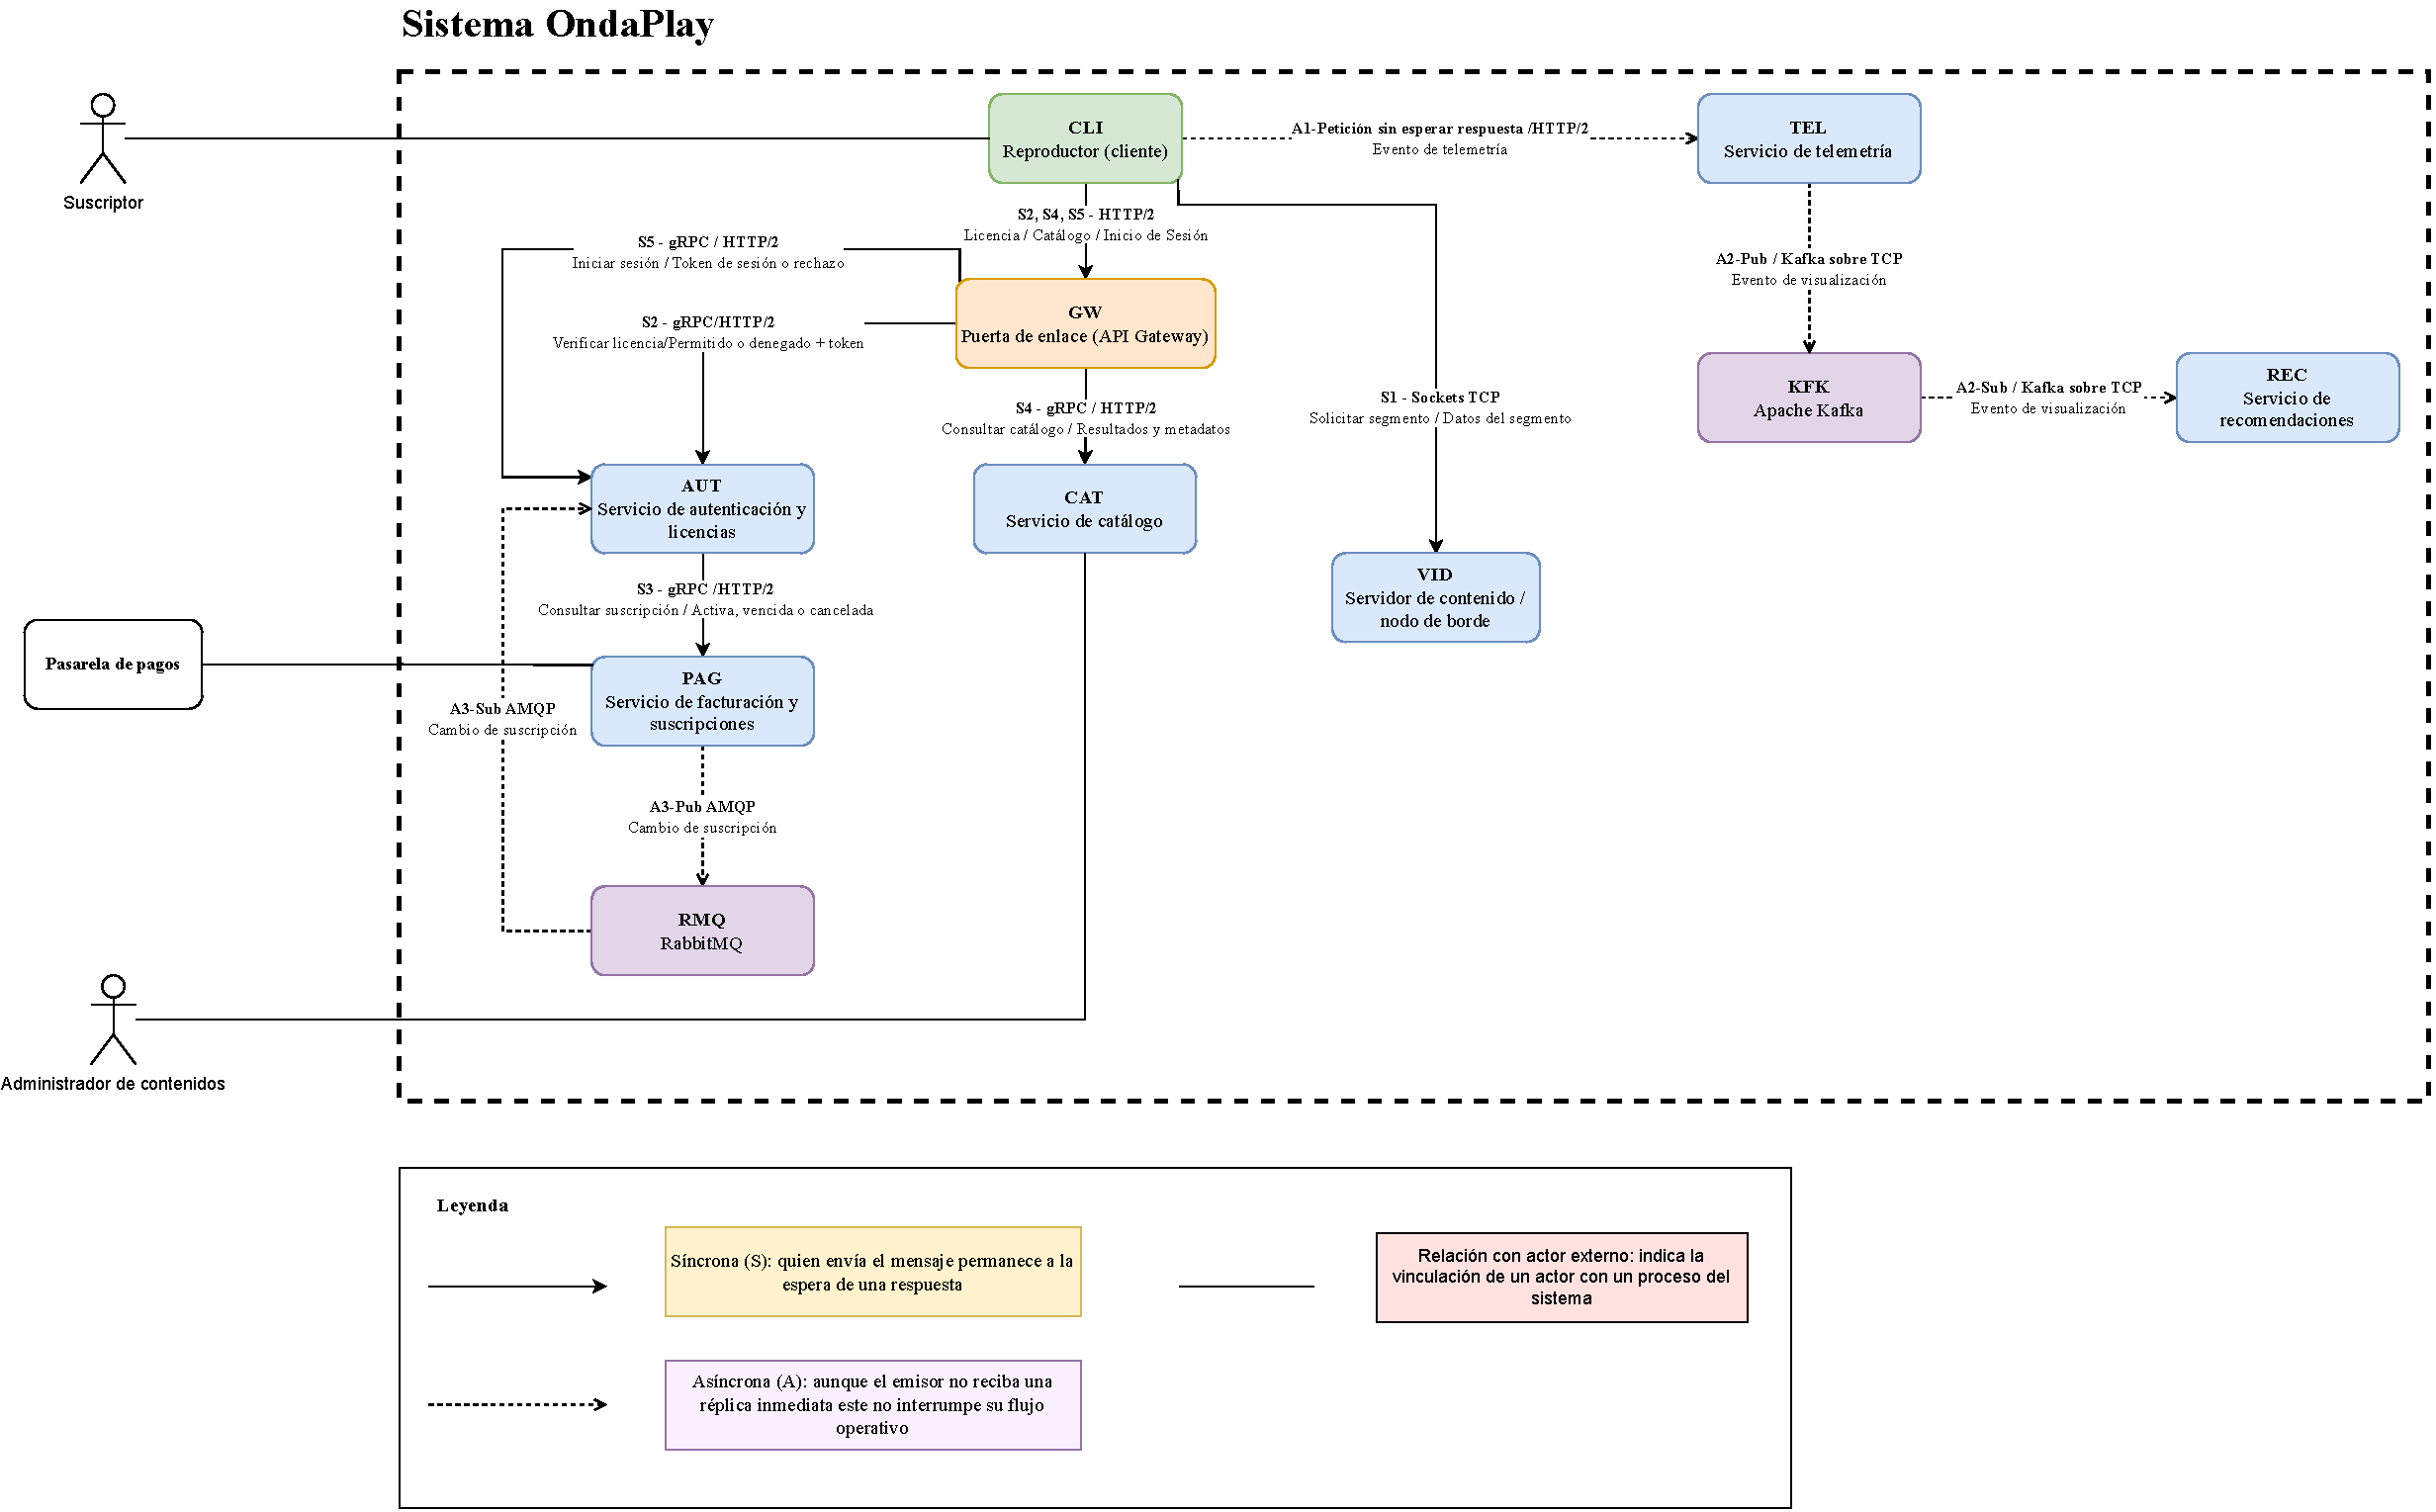
\includegraphics[width=\textwidth]{comunicacion}
    \caption{Comunicación entre los procesos y actores externos de OndaPlay}
    \label{fig:diagrama}
\end{figure}

\subsection{Componentes del sistema}

Los componentes se identifican mediante códigos que
permiten reconocerlos dentro del diagrama. CLI representa
al reproductor (cliente), desde el cual el suscriptor accede
a la plataforma, mientras que GW corresponde a la puerta de enlace que recibe y
dirige las solicitudes hacia los servicios internos.

AUT se encarga de la autenticación y las licencias, CAT representa el servicio de catálogo, VID corresponde
al servidor de contenido o nodo de borde, y PAG identifica al servicio de
facturación y suscripciones.

También se incluyen TEL, encargado de la telemetría, y
REC, representa al servicio de recomendaciones de contenido.
Para la comunicación asíncrona se utilizan KFK (Apache Kafka) y RMQ (RabbitMQ), estos permiten intercambiar
mensajes entre los procesos.

Fuera de la frontera del sistema se encuentran tres actores externos: Suscriptor (utiliza el reproductor), Administrador de contenidos
(interactúa con el catálogo) y Pasarela de pagos (se comunica con el servicio de facturación y suscripciones).

\subsection{Notación utilizada}

Las flechas indican la dirección en la que se envían
los mensajes entre los procesos. Se utilizan líneas
continuas para representar las comunicaciones síncronas,
en las que el emisor espera una respuesta antes de
continuar, y líneas discontinuas para las comunicaciones
asíncronas, en las que el emisor no necesita esperar
una respuesta inmediata.

Cada interacción se identifica con un código. La letra
S seguida de un número corresponde a una comunicación
síncrona, mientras que la letra A es utilizada para una
comunicación asíncrona. Junto a cada etiqueta se detallan los datos intercambiados, el mecanismo de
comunicación y el protocolo utilizado.

Las relaciones con los actores externos se representan mediante líneas continuas sin puntas de flecha en ninguno de sus extremos
y sin identificadores S o A (como los mencionados anteriormente). Estas líneas permiten distinguir la participación de los actores
de las comunicaciones entre los procesos internos de OndaPlay

\subsection{Lectura del diagrama}

En las comunicaciones síncronas representadas, S1 corresponde a la solicitud de segmentos de video desde el reproductor
(CLI) directamente al servidor de contenido (VID), sin pasar por la puerta de enlace (GW). Esta comunicación utiliza 
sockets TCP.

La interacción S2 corresponde a la comunicación entre GW y AUT para verificar las licencias. En S3, AUT consulta a PAG para comprobar el estado de la suscripción, 
mientras que S4 permite a GW solicitar información del catálogo a CAT.
Por su parte, S5 representa el inicio de sesión. La solicitud se envía desde CLI hacia GW y luego a AUT, 
donde se realiza la autenticación y se devuelve un token de sesión o un rechazo. Las interacciones S2, S3, S4 y S5 utilizan gRPC sobre HTTP/2.

En las comunicaciones asíncronas, A1 representa el envío de eventos de telemetría desde CLI hacia TEL. En A2, TEL publica eventos de visualización mediante Kafka (KFK), 
que posteriormente son consumidos por REC para generar recomendaciones.

Finalmente, A3 representa la comunicación desde PAG hacia AUT mediante RabbitMQ (RMQ), utilizada para informar los cambios en las suscripciones. Los mecanismos y protocolos de estas interacciones asíncronas se detallan en la Sección 4.
\section{Interacciones síncronas: sockets y RPC}

\section{Interacciones asíncronas y tolerancia a fallos}

\section{Declaración de uso de inteligencia artificial}

\begin{table}[H]
  \centering
  \small
  \caption{Herramientas de inteligencia artificial usadas como apoyo}
  \label{tab:declaracion-ia}
  \begin{tabularx}{\textwidth}{@{}>{\raggedright\arraybackslash}p{2.5cm}>{\raggedright\arraybackslash}p{1.7cm}>{\raggedright\arraybackslash}X>{\raggedright\arraybackslash}X@{}}
    \toprule
    \textbf{Herramienta} & \textbf{Versión} & \textbf{Para qué se usó} & \textbf{Cómo se verificó lo obtenido} \\
    \midrule
    Claude Code, aplicación de escritorio (Mario Castro) &
    Claude Fable 5.2 &
    Crear el repositorio con la plantilla LaTeX del curso, las ramas y las
    invitaciones. Resumir la guía y la rúbrica y armar el plan de trabajo.
    Proponer una lista inicial de procesos con códigos cortos. Redactar los
    mensajes de coordinación del grupo. Generar la carátula del SGA. Dar los
    comandos de Git y resolver errores. Revisar las secciones 1 y 4 y el
    archivo del diagrama, y compilar el informe para buscar desbordes.
    Listar estos usos a partir del registro de la sesión. &
    Los comandos los ejecutó el integrante y el resultado se comprobó en
    GitHub. La lista de procesos se contrastó con el Anexo A de la rúbrica:
    se cambió por los siete procesos del enunciado y solo se conservaron los
    códigos. Cada observación de las revisiones se comprobó en el enunciado
    o en la sección citada antes de cambiar el texto. La compilación se
    repite con los comandos del README. \\
    \addlinespace
    Claude, aplicación de escritorio, modo Cowork (Dayver Rivas) &
    Claude Opus 5.5 &
    Explicar la tarea, la rúbrica y conceptos de mensajería: Kafka y
    RabbitMQ, colas y pub/sub, ACK, DLQ, retención y offset. Armar la
    plantilla vacía de la sección 4. Instalar Git y dar sus comandos.
    Revisar el texto de la sección 4 contra la rúbrica, el Anexo A y la
    sección 3. Probar la compilación. &
    Las interacciones A1, A2 y A3 se contrastaron con R3, R4, R5 y F2 del
    Anexo A. Los tiempos de A3 se compararon con los de S3 en la sección 3.
    El archivo se compiló en el equipo del integrante. \\
    \addlinespace
    GitHub Copilot en Visual Studio Code 1.145.3 (Dayver Rivas) &
    1.0.103 &
    Sugerencias automáticas al escribir. Se aceptó una por error. &
    La sugerencia se borró, se desactivó la extensión y se releyó el
    archivo completo. \\
    \bottomrule
  \end{tabularx}
\end{table}

\printbibliography[heading=bibintoc,title={Referencias}]

\end{document}
